%!TEX root = ../../master.tex
\chapter{Physical Design}
\label{appendix_physical_design}
The cluster has been designed to look like a scale-model of a server rack in a datacenter. This appendix will present the sketches, 3D models, technical drawings and final physical layouts.


\section*{Sketches}
In order to design the cluster to fit the size of a Raspberry Pi several sketches and drafts were made. Figure~\ref{fig:sketches} (a) shows how the the cable holes were designed for the layers with Raspberry Pis. Two different layers were made: a layer serving as the bottom/top layers and a layer with holes to mount a Raspberry Pi and holes for power and network cables. Figure~\ref{fig:sketches} (b) shows the first version of the Raspberry Pi layer with the location of the switch shown underneath. The switch's cable plugs were later moved to the back because we found a smaller switch than expected. \\

\begin{figure}[H]%
    \centering
    \subfloat[Sketch of Raspberry Pi on layer]{{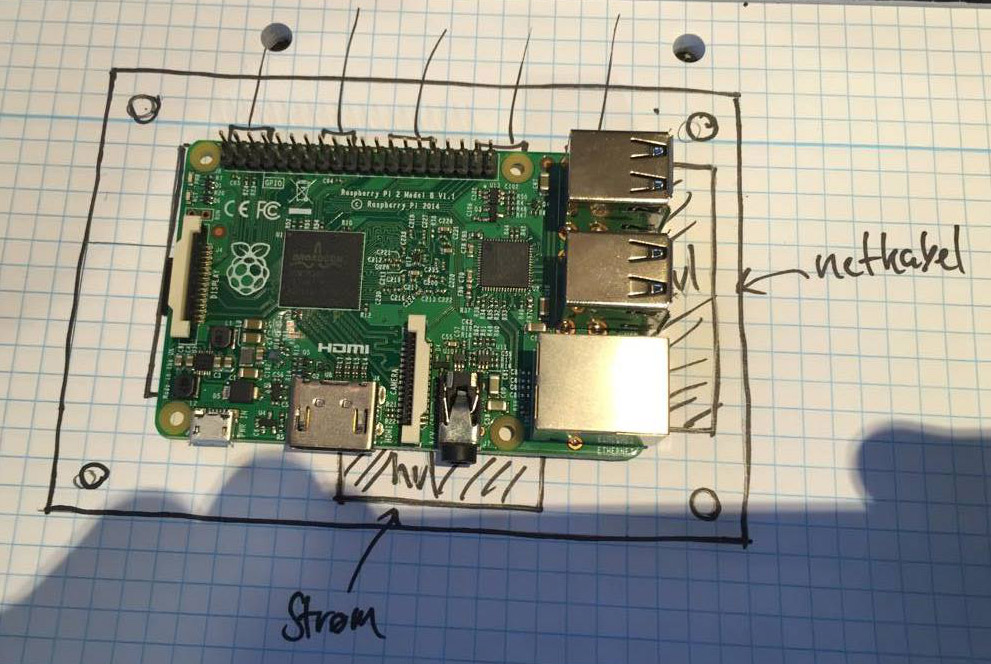
\includegraphics[width=7cm]{figures/cluster/drawing_1} }}%
      \qquad
    \subfloat[Sketch of Raspberry Pi layer with switch]{{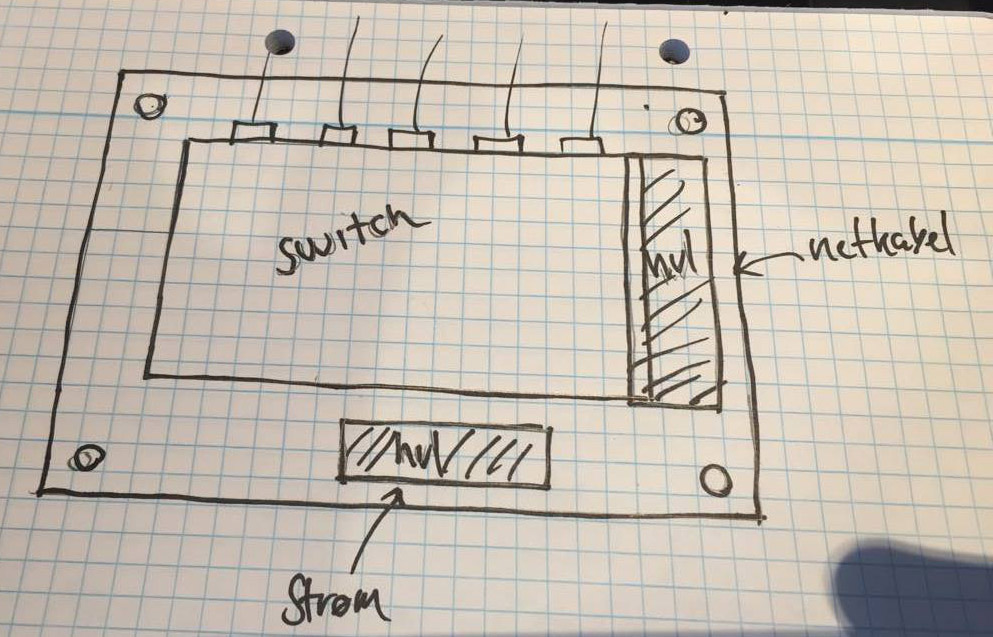
\includegraphics[width=7cm]{figures/cluster/drawing_2} }}%
    \caption{Sketches}%
    \label{fig:sketches}%
\end{figure}


\section*{3D Models}
Figure~\ref{fig:cluster_3d_model} shows the designed 3D model before components were bought. The switch was replaced with another model, but the rest of the model is identical to the clusters we have build. More information and 3D models can be found at \url{http://rpi-cloud.com/guide-how-to-build-a-raspberry-pi-cluster/}.

\begin{figure}[H]
	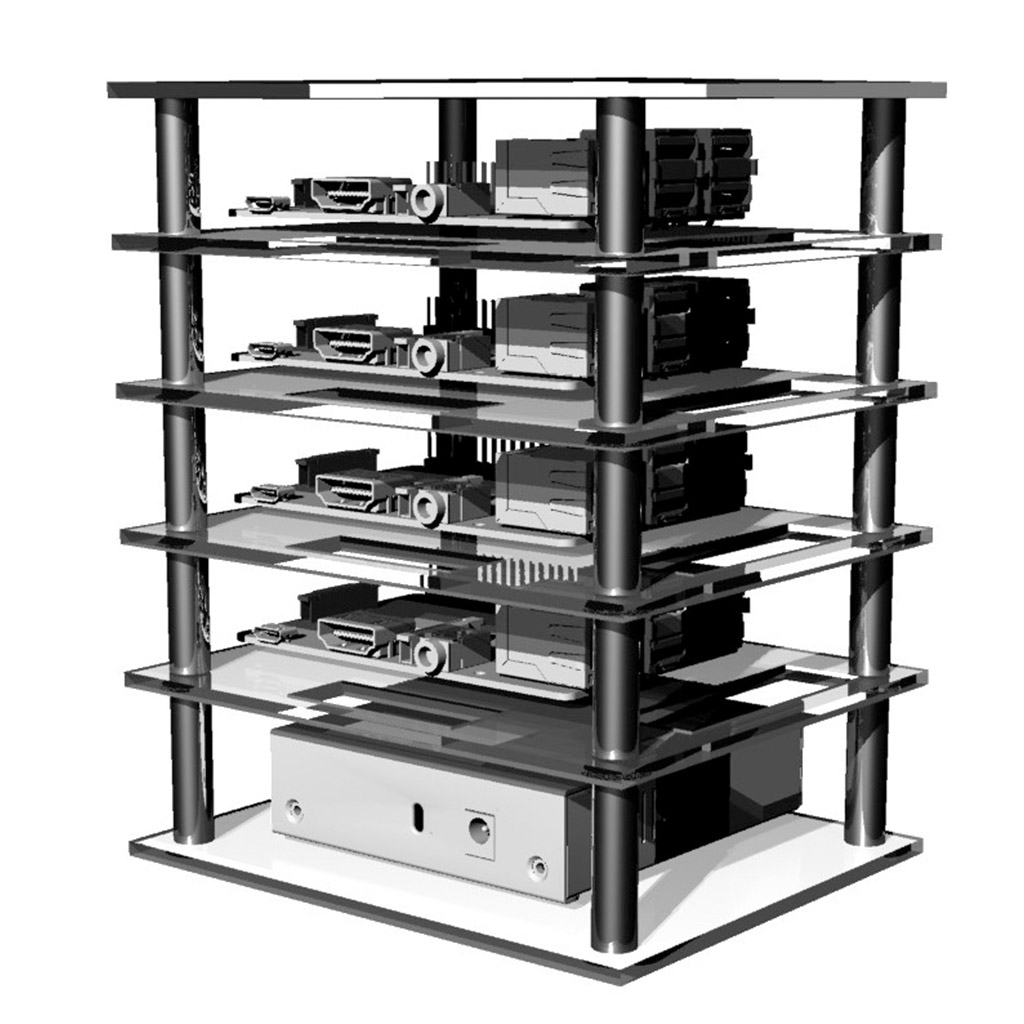
\includegraphics[width=5cm]{figures/cluster/cluster3d_back}
	\centering
	\caption{Cluster 3D Model}
	\label{fig:cluster_3d_model}
\end{figure}



\section*{Technical Drawings}

\begin{figure}[H]
	\centering
	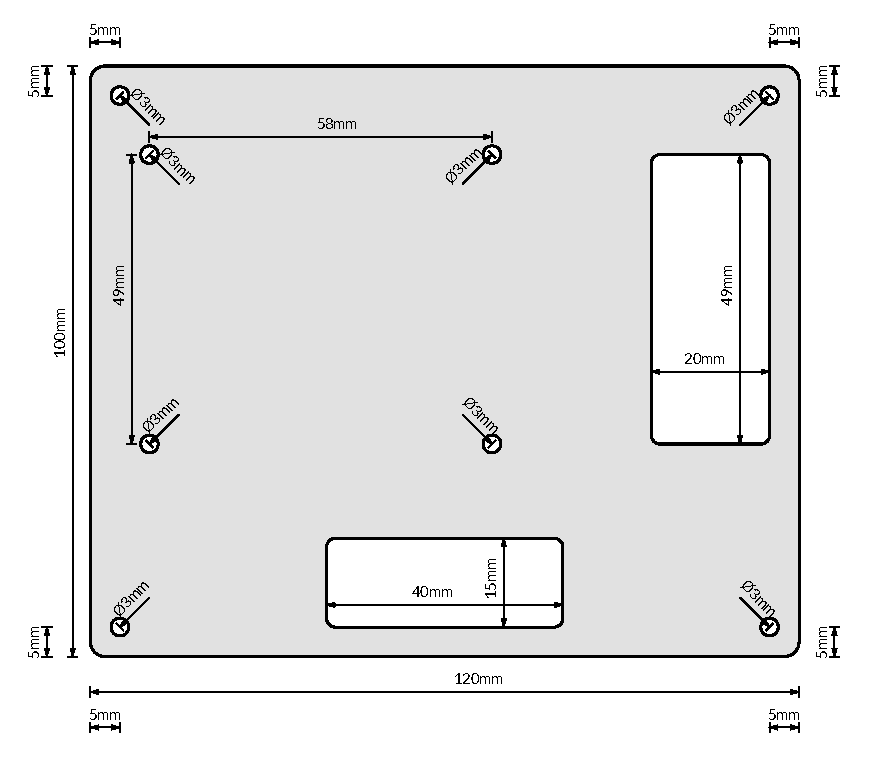
\includegraphics[width=16cm]{figures/cluster/raspberry_layer}
	\caption{Raspberry Pi Layer 1:1}
	\label{fig:cluster_raspberry_layer}
\end{figure}

\newpage

\begin{figure}[H]
	\centering
	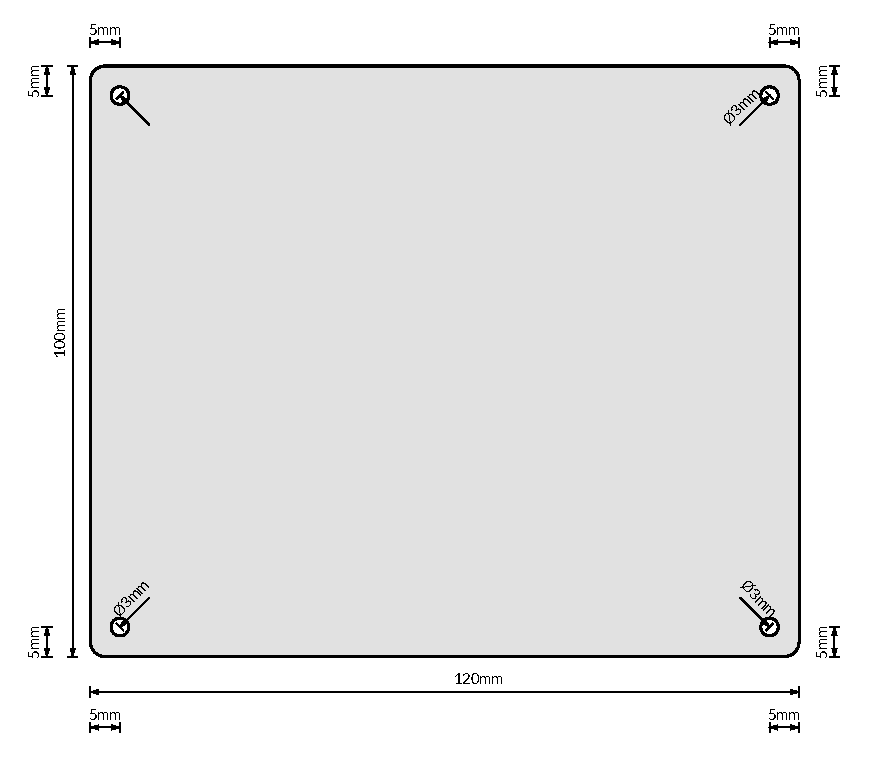
\includegraphics[width=16cm]{figures/cluster/top_bottom_layer}
	\caption{Top/bottom layer 1:1}
	\label{fig:cluster_top_bottom_layer}
\end{figure}

\newpage
\section*{Final Physical Layouts}
The fabricated cluster is shown in the following images.

\begin{figure}[H]%
    \centering
    \subfloat[Front]{{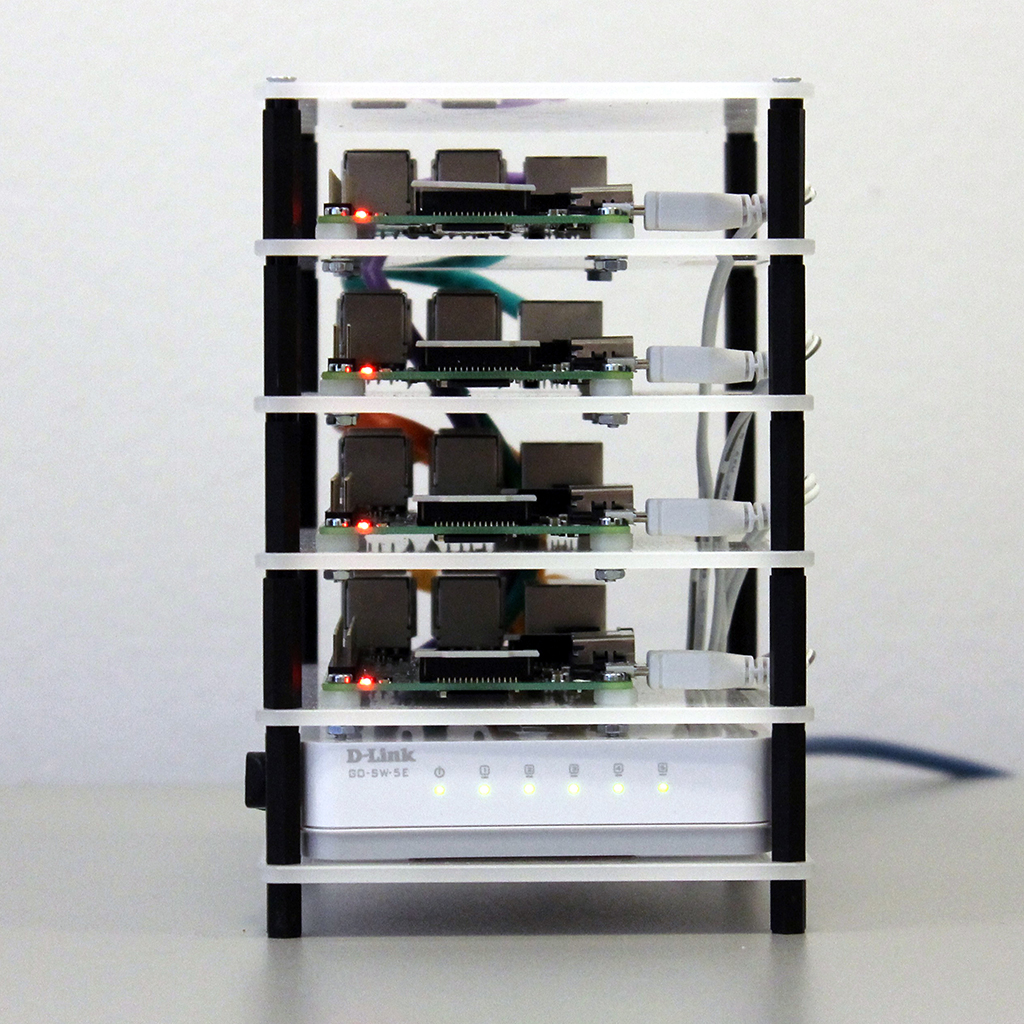
\includegraphics[width=7cm]{figures/cluster/front} }}%
      \qquad
    \subfloat[Back]{{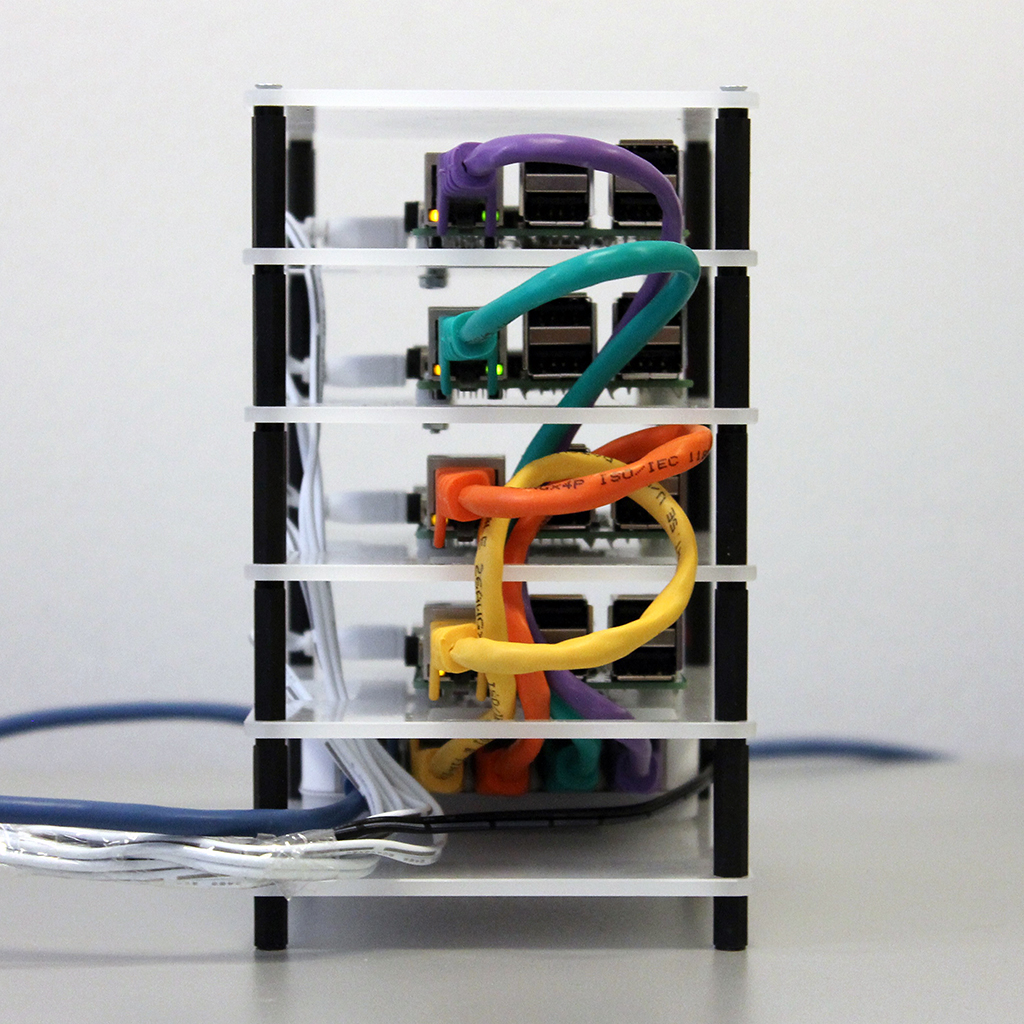
\includegraphics[width=7cm]{figures/cluster/back} }}%
          \qquad
    \subfloat[Left]{{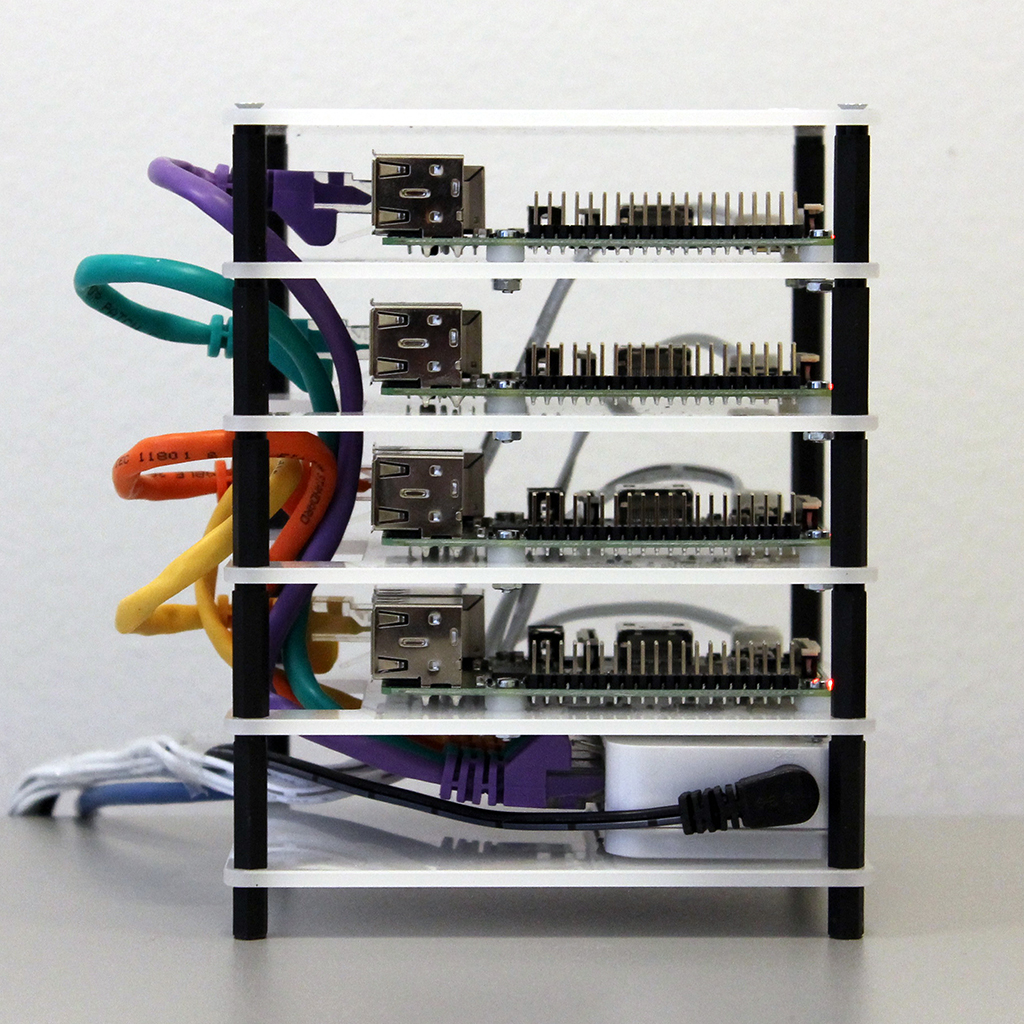
\includegraphics[width=7cm]{figures/cluster/left} }}%
          \qquad
    \subfloat[Right]{{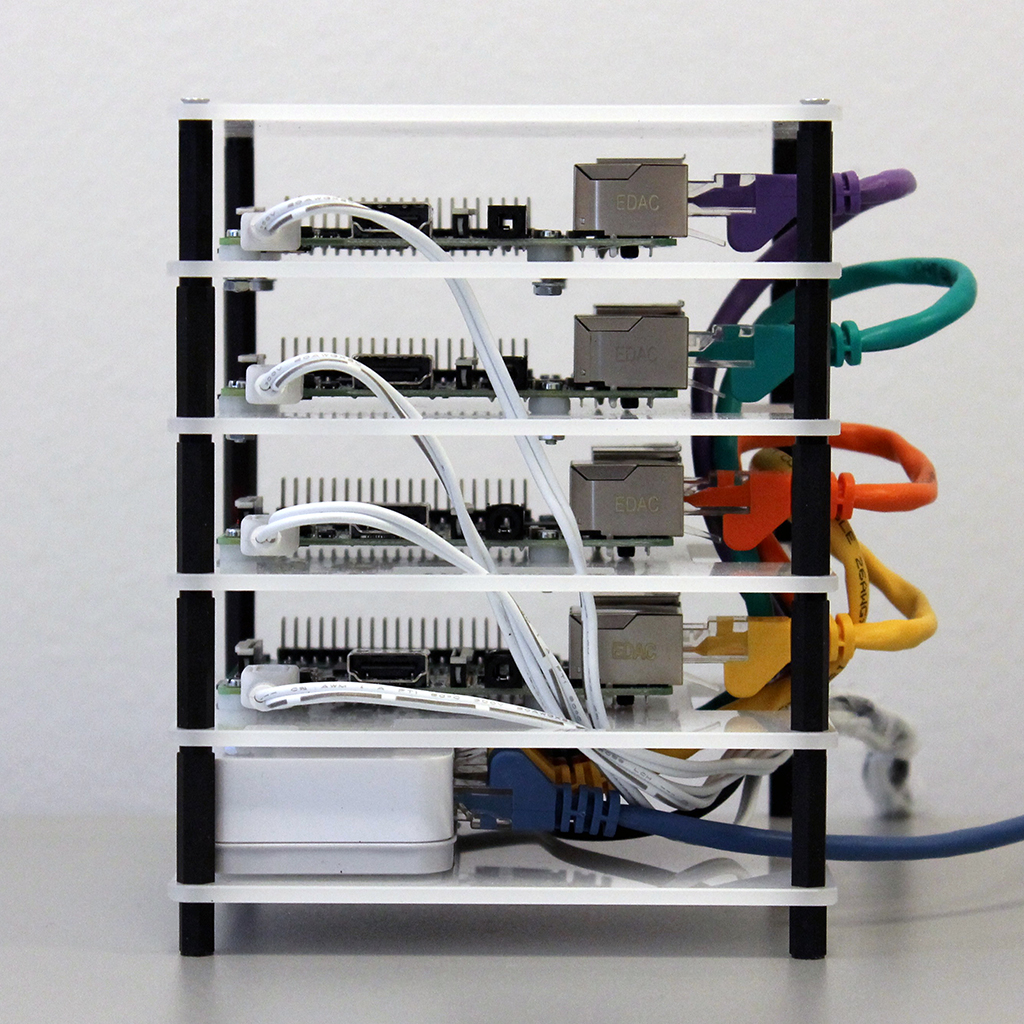
\includegraphics[width=7cm]{figures/cluster/right} }}%
    \caption{KubeCloud}%
    \label{fig:kubecloud_physical}%
\end{figure}
